\documentclass[11pt]{article}

% ----------------------------------------------------------
% PACKAGES
% ----------------------------------------------------------
\usepackage[T1]{fontenc}
\usepackage[utf8]{inputenc}
\usepackage{lmodern}
\usepackage[margin=1in]{geometry}
\usepackage{amsmath, amssymb}

\usepackage{graphicx}
\usepackage{xcolor}
\usepackage{booktabs}
\usepackage{enumitem}

% TikZ + PGFPLOTS (REQUIRED FOR FIGURES)
\usepackage{tikz}
\usepackage{pgfplots}
\pgfplotsset{compat=1.18}
\usepgfplotslibrary{groupplots}

\usepackage{framed}
\usepackage{setspace}
\usepackage{microtype}
\usepackage[hidelinks]{hyperref}
\usepackage[authoryear]{natbib}

% ----------------------------------------------------------
% CUSTOM MACROS (shared notation)
% ----------------------------------------------------------
% ==========================================================
% EB-PAPERS: CANONICAL MACROS / COMMANDS
% Forecast Readiness Framework (FRF) / Electric Barometer
% ==========================================================
% Goals:
% - One meaning per symbol.
% - Shared across all papers/notes/briefs.
% - Backwards-compatible aliases.
% - Avoid redefinition errors via \providecommand.
% ==========================================================

% ----------------------------------------------------------
% Core framework / artifacts
% ----------------------------------------------------------
\providecommand{\FRF}{\ensuremath{\mathrm{FRF}}}
\providecommand{\FRS}{\ensuremath{\mathrm{FRS}}}

\providecommand{\FPC}{\ensuremath{\mathrm{FPC}}}
\providecommand{\DQC}{\ensuremath{\mathrm{DQC}}}
\providecommand{\Governance}{\ensuremath{\mathrm{Governance}}}
\providecommand{\GovernanceDecision}{\ensuremath{\mathrm{GovernanceDecision}}}

\providecommand{\RAL}{\ensuremath{\mathrm{RAL}}}

% Readiness primitives / governance vocabulary
\providecommand{\ReadinessPrimitive}{\ensuremath{\mathrm{RP}}}

% Limited-Time Offers
\providecommand{\LTO}{\ensuremath{\mathrm{LTO}}}
\providecommand{\LTOs}{\ensuremath{\mathrm{LTOs}}}

% ----------------------------------------------------------
% Core metrics (upright math)
% ----------------------------------------------------------
\providecommand{\CWSL}{\ensuremath{\mathrm{CWSL}}}
\providecommand{\CWSLR}{\ensuremath{\mathrm{CWSLR}}} % named artifact in prose
\providecommand{\NSL}{\ensuremath{\mathrm{NSL}}}
\providecommand{\UD}{\ensuremath{\mathrm{UD}}}
\providecommand{\HR}{\ensuremath{\mathrm{HR}}}
\providecommand{\HRtau}{\ensuremath{\mathrm{HR}@\tau}}

% FRS sub-terms
\providecommand{\CWSLscaled}{\ensuremath{\mathrm{CWSL}_{\mathrm{scaled}}}}
\providecommand{\CWSLmax}{\ensuremath{\mathrm{CWSL}_{\max}}}

% Legacy HR macro names
\providecommand{\HRAT}{\ensuremath{\mathrm{HR@\tau}}}
\providecommand{\tauTol}{\ensuremath{\tau}}
\providecommand{\tauop}{\ensuremath{\tau}}

% ----------------------------------------------------------
% Indexing and sets
% ----------------------------------------------------------
\providecommand{\Iset}{\ensuremath{I}}
\providecommand{\Tset}{\ensuremath{T}}

\providecommand{\entity}{\ensuremath{i}}
\providecommand{\timeindex}{\ensuremath{t}}

% Back-compat index shorthands
\providecommand{\iidx}{\entity}
\providecommand{\tidx}{\timeindex}

% Summation shorthand
\providecommand{\sumit}{\ensuremath{\sum_{\entity \in \Iset} \sum_{\timeindex \in \Tset}}}

% Optional sizes / counts
\providecommand{\Tsize}{\ensuremath{|\Tset|}}
\providecommand{\nobs}{\ensuremath{N}}

% ----------------------------------------------------------
% Forecast / demand notation
% ----------------------------------------------------------
\providecommand{\y}{\ensuremath{y}}
\providecommand{\yhat}{\ensuremath{\hat{y}}}

\providecommand{\yit}{\ensuremath{y_{\entity\timeindex}}}
\providecommand{\yhatit}{\ensuremath{\hat{y}_{\entity\timeindex}}}

% Common residuals / errors
\providecommand{\errit}{\ensuremath{e_{\entity\timeindex}}}
\providecommand{\resit}{\errit} % alias
\providecommand{\absit}{\ensuremath{\left|\yhatit - \yit\right|}}
\providecommand{\abserrit}{\absit} % alias

% Explicit residual definition macro (optional)
\providecommand{\resdef}{\ensuremath{\errit = \yit - \yhatit}}

% ----------------------------------------------------------
% Shortfall / overbuild decomposition
% ----------------------------------------------------------
\providecommand{\shortfall}{\ensuremath{s}}
\providecommand{\overbuild}{\ensuremath{o}}

\providecommand{\sit}{\ensuremath{s_{\entity\timeindex}}}
\providecommand{\oit}{\ensuremath{o_{\entity\timeindex}}}

% Positive-part operator (canonical name)
\providecommand{\pospart}[1]{\left(#1\right)_{+}}

% Explicit decompositions
\providecommand{\shortfalldef}{\ensuremath{\sit = \pospart{\yit - \yhatit}}}
\providecommand{\overbuilddef}{\ensuremath{\oit = \pospart{\yhatit - \yit}}}

% Back-compat convenience symbols used in some notes
\providecommand{\sdepth}{\shortfall} % UD paper convenience

% ----------------------------------------------------------
% Indicators / expectations / operators
% ----------------------------------------------------------
% Canonical indicator: \Ind{event}
\providecommand{\Ind}{\ensuremath{\mathbb{I}}}
\providecommand{\indicator}[1]{\ensuremath{\mathbf{1}\{#1\}}} % prose-friendly alternative

% Back-compat: some notes used \Indicator (capital I). Keep as an alias to the
% canonical \Ind to avoid duplicate meanings.
\providecommand{\Indicator}{\Ind}

% If you want function-style indicator without braces: \Ind\!(event)
% Keep as \Ind and let authors decide.
\providecommand{\E}{\ensuremath{\mathbb{E}}}

\providecommand{\abs}[1]{\left|#1\right|}
\providecommand{\card}[1]{\left|#1\right|}

% ----------------------------------------------------------
% Cost parameters + cost ratio calibration (CWSLR note)
% ----------------------------------------------------------
% IMPORTANT: Canonical costs are subscripted (c_u, c_o). This avoids
% collisions with superscript variants.
\providecommand{\cu}{\ensuremath{c_u}}
\providecommand{\co}{\ensuremath{c_o}}

% Entity-specific costs
\providecommand{\cui}{\ensuremath{c_{u,\entity}}}
\providecommand{\coi}{\ensuremath{c_{o,\entity}}}

% Cost ratio
\providecommand{\R}{\ensuremath{R}}
\providecommand{\Ri}{\ensuremath{R_{\entity}}}
\providecommand{\Rdef}{\ensuremath{R = \cu/\co}}

% Aggregate under/over cost functions (used in calibration prose)
\providecommand{\UnderCost}{\ensuremath{\mathrm{UnderCost}}}
\providecommand{\OverCost}{\ensuremath{\mathrm{OverCost}}}

% Candidate grid
\providecommand{\Rgrid}{\ensuremath{\mathcal{R}}}

% Calibrated selections
\providecommand{\Rstar}{\ensuremath{R^{\ast}}}
\providecommand{\Rist}{\ensuremath{R^{\ast}_{\entity}}}

% CWSL as a function of R (notation)
\providecommand{\CWSLofR}{\ensuremath{\CWSL(\R)}}
\providecommand{\CWSLofRi}{\ensuremath{\CWSL(\Ri)}}

% Balance-based selection operator (kept as a macro because you used it)
\providecommand{\Rbalance}{%
\ensuremath{%
\arg\min_{\R \in \Rgrid}\left|\UnderCost(\R) - \OverCost(\R)\right|%
}%
}

% Back-compat (older notes used superscripts c^u / c^o)
\providecommand{\cuSup}{\ensuremath{c^{u}}}
\providecommand{\coSup}{\ensuremath{c^{o}}}
\providecommand{\cuiSup}{\ensuremath{c^{u}_{\entity}}}
\providecommand{\coiSup}{\ensuremath{c^{o}_{\entity}}}

% ----------------------------------------------------------
% HR@tau scanning / calibration (HRtau note)
% ----------------------------------------------------------
\providecommand{\tauval}{\ensuremath{\tau}}
\providecommand{\tauv}{\tauval}
\providecommand{\taui}{\ensuremath{\tau_{\entity}}}

% Candidate tolerance grid
\providecommand{\TauGrid}{\ensuremath{\mathcal{T}}}

% Calibrated tolerances
\providecommand{\taustar}{\ensuremath{\tau^{\ast}}}
\providecommand{\taustari}{\ensuremath{\tau^{\ast}_{\entity}}}

% Target hit-rate (if used)
\providecommand{\hstar}{\ensuremath{h^{\ast}}}

% Hit indicator definition helpers
\providecommand{\Hitit}{\ensuremath{h_{\entity\timeindex}}}
\providecommand{\HitDef}{\ensuremath{\Hitit = \Ind\!\left(\absit \le \tauval\right)}}

% HR as a function of tau
\providecommand{\HRoftau}{\ensuremath{\HR(\tauval)}}
\providecommand{\HRtauoftau}{\ensuremath{\HRtau(\tauval)}}

% Optional utility selection helpers
\providecommand{\lambdau}{\ensuremath{\lambda}}
\providecommand{\taumax}{\ensuremath{\tau_{\max}}}
\providecommand{\Utility}{\ensuremath{\mathcal{U}}}
\providecommand{\UtilityDef}{\ensuremath{\Utility(\tauval) = \HR(\tauval) - \lambdau \cdot (\tauval/\taumax)}}

% Governance guards
\providecommand{\taufloor}{\ensuremath{\tau_{\min}}}
\providecommand{\taucap}{\ensuremath{\tau_{\mathrm{cap}}}}
\providecommand{\nmin}{\ensuremath{n_{\min}}}

% ----------------------------------------------------------
% DQC / snapping / quantization (DQC note)
% ----------------------------------------------------------
\providecommand{\gunit}{\ensuremath{g}}
\providecommand{\guniti}{\ensuremath{g_{\entity}}}

\providecommand{\ygrid}{\ensuremath{\tilde{y}}}
\providecommand{\ygridit}{\ensuremath{\tilde{y}_{\entity\timeindex}}}

\providecommand{\yhatgrid}{\ensuremath{\tilde{\hat{y}}}}
\providecommand{\yhatgridit}{\ensuremath{\tilde{\hat{y}}_{\entity\timeindex}}}

\providecommand{\snap}{\ensuremath{\mathcal{S}}}
\providecommand{\snaphatdef}{\ensuremath{\yhatgridit = \snap_{\gunit}\!\left(\yhatit\right)}}
\providecommand{\snapydef}{\ensuremath{\ygridit = \snap_{\gunit}\!\left(\yit\right)}}

\providecommand{\residit}{\ensuremath{r_{\entity\timeindex}}}
\providecommand{\residdef}{\ensuremath{\residit = \yit - \ygridit}}

\providecommand{\MAD}{\ensuremath{\mathrm{MAD}}}
\providecommand{\IQR}{\ensuremath{\mathrm{IQR}}}

\providecommand{\multirate}{\ensuremath{\rho}}
\providecommand{\multiratei}{\ensuremath{\rho_{\entity}}}

\providecommand{\DeltaStar}{\ensuremath{\Delta^{\ast}}}

\providecommand{\Pset}{\ensuremath{\mathcal{P}}}
\providecommand{\packunit}{\ensuremath{p}}
\providecommand{\packuniti}{\ensuremath{p_{\entity}}}

% DQC classes
\providecommand{\ContinuousLike}{\textsc{Continuous-like}}
\providecommand{\Quantized}{\textsc{Quantized}}
\providecommand{\PiecewisePacked}{\textsc{Piecewise-packed}}

% FPC classes
\providecommand{\Compatible}{\textsc{Compatible}}
\providecommand{\Marginal}{\textsc{Marginal}}
\providecommand{\Incompatible}{\textsc{Incompatible}}

% ----------------------------------------------------------
% RAL shorthands used in notes
% ----------------------------------------------------------
\providecommand{\alphaadj}{\ensuremath{\alpha}}

% RAL operator (functional form)
\providecommand{\RALop}{\ensuremath{\mathcal{R}_{\alphaadj}}}

\providecommand{\yhatadjit}{\ensuremath{\hat{y}^{(\alphaadj)}_{\entity\timeindex}}}
\providecommand{\yhatadjdef}{\ensuremath{\yhatadjit = (1+\alphaadj)\,\yhatit}}

\providecommand{\dNSL}{\ensuremath{\Delta \NSL}}
\providecommand{\dHRtau}{\ensuremath{\Delta \HRtau}}
\providecommand{\dCWSL}{\ensuremath{\Delta \CWSL}}

% ----------------------------------------------------------
% Governance policy handles
% ----------------------------------------------------------
\providecommand{\TauPolicy}{\ensuremath{\mathrm{TauPolicy}}}
\providecommand{\RALPolicy}{\ensuremath{\mathrm{RALPolicy}}}
\providecommand{\UnitPolicy}{\ensuremath{\mathrm{UnitPolicy}}}

\providecommand{\GovernanceStatus}{\ensuremath{\mathrm{GovernanceStatus}}}
\providecommand{\Green}{\textsc{Green}}
\providecommand{\Yellow}{\textsc{Yellow}}
\providecommand{\Red}{\textsc{Red}}

\providecommand{\RawUnits}{\textsc{Raw}}
\providecommand{\SnappedUnits}{\textsc{Snapped}}

% ----------------------------------------------------------
% LTO paper specifics
% ----------------------------------------------------------
\providecommand{\ltoOn}{\ensuremath{z_{\timeindex}}}
\providecommand{\ltoPhase}{\ensuremath{\phi_{\timeindex}}}
\providecommand{\qprod}{\ensuremath{\mathrm{QP}}}

% ----------------------------------------------------------
% Frontmatter helpers
% ----------------------------------------------------------
\providecommand{\keywords}[1]{%
\par\noindent\textbf{Keywords: }#1\par
}

% ----------------------------------------------------------
% Prose shorthands
% ----------------------------------------------------------
\providecommand{\ie}{i.e.\ }
\providecommand{\eg}{e.g.\ }

% ==========================================================
% END
% ==========================================================


% ----------------------------------------------------------
% PDF METADATA
% ----------------------------------------------------------
\hypersetup{
    pdftitle={Cost-Weighted Service Loss (\CWSL): An Asymmetric Cost Metric for Forecast Evaluation},
    pdfauthor={Kyle Corrie},
    colorlinks=true,
    linkcolor=blue,
    citecolor=blue,
    urlcolor=blue
}

% ----------------------------------------------------------
% TITLE BLOCK
% ----------------------------------------------------------
\title{
\textbf{Cost-Weighted Service Loss (\CWSL):}\\[4pt]
{\large An Asymmetric Cost Metric for Forecast Evaluation}
}

\author{
  Kyle Corrie\\[4pt]
  \small Forecast Readiness Framework (FRF)\\
  \small Electric Barometer Series
}

\date{December 2025\\[4pt]
\small Technical Note --- Electric Barometer Series\\
Version 1.0}

% ==================================================
\begin{document}

\maketitle

% ----------------------------------------------------------
% ABSTRACT
% ----------------------------------------------------------
\begin{abstract}
Cost-Weighted Service Loss (CWSL) quantifies the asymmetric operational impact 
of forecast error by applying explicit penalties to underbuild and overbuild.
Traditional symmetric accuracy metrics treat positive and negative deviations 
equivalently, but in many operational environments—production, staffing, 
logistics, inventory, and energy systems—the cost of underforecasting often 
significantly outweighs the cost of surplus. CWSL encodes this asymmetry 
directly and normalizes by realized demand, making the metric interpretable as 
the effective fraction of throughput “lost’’ due to misalignment between 
forecasted and actual values. This technical note presents the formal definition, 
properties, motivation, and illustrative examples of CWSL, and outlines how it 
supports readiness-oriented forecast evaluation within the Forecast Readiness 
Framework.
\end{abstract}

% ----------------------------------------------------------
% ORDERED SECTION INPUTS (Technical Note Schema)
% ----------------------------------------------------------
% ==========================================================
% 010_overview.tex
% Overview
% ==========================================================

\section{Overview}
\label{sec:governance_overview}

Modern operational forecasting systems increasingly embed automated control
levers, tolerance-based evaluation, and asymmetric cost tradeoffs directly into
decision workflows. In such settings, analytic diagnostics alone are
insufficient. What ultimately matters is not whether a forecast appears
reasonable, but whether a downstream action is \emph{structurally admissible},
\emph{policy-compliant}, and \emph{accountable}.

Within the Electric Barometer framework, this responsibility is assigned to
\emph{Governance}. Governance is the final decision layer that binds structural
diagnostics into an authoritative operational outcome. It does not generate new
signals, optimize objectives, or reinterpret performance. Instead, it resolves
diagnostic inputs into a single, enforceable policy decision.

This technical note formalizes governance as a deterministic \emph{decision
contract}. Given a fixed set of diagnostic inputs and thresholds, governance
produces exactly one authoritative artifact that specifies:
\begin{itemize}[leftmargin=1.5em]
  \item the admissible unit system for interpretation,
  \item the authoritative tolerance semantics,
  \item the allowability of readiness adjustment,
  \item and an explicit governance status.
\end{itemize}

Governance consumes—but does not redefine—two upstream diagnostics:
\begin{itemize}[leftmargin=1.5em]
  \item \textbf{Demand Quantization Compatibility (DQC)}, which determines whether
        realized demand admits continuous interpretation or requires discrete,
        grid-aware semantics; and
  \item \textbf{Forecast Primitive Compatibility (FPC)}, which determines whether
        a forecast primitive can respond coherently to readiness adjustment under
        admissible perturbations.
\end{itemize}

Crucially, governance does not average, negotiate, or arbitrate between these
diagnostics. It enforces strict exclusivity: one unit system governs, one
diagnostic interpretation is authoritative, and one readiness policy applies.
When required inputs are missing or incompatible, governance fails explicitly
rather than degrading silently.

The purpose of this design is closure. Governance exists to \emph{terminate
interpretation, not extend it}: once a \texttt{GovernanceDecision} is issued, no
further diagnostic reasoning is admissible.

By enforcing this closure, governance prevents common operational failure modes
such as:
\begin{itemize}[leftmargin=1.5em]
  \item mixing raw and snapped evaluation semantics,
  \item interpreting tolerances smaller than realizable demand increments,
  \item applying readiness adjustments that cannot be operationally executed.
\end{itemize}

This note describes the governance contract, the structure of the decision
artifact it emits, the deterministic logic by which decisions are made, and the
interpretive boundaries that preserve accountability. Together with the DQC and
FPC technical notes, it completes the Electric Barometer framework by ensuring
that readiness decisions are not only cost-aware or service-aware, but
\emph{structurally valid, auditable, and enforceable by design}.

% ----------------------------------------------------------
% DEFINITION
% ----------------------------------------------------------
\section{Definition}

The Readiness Adjustment Layer (RAL) is defined as a deterministic operator that
maps a baseline forecast to an adjusted forecast in order to reduce
decision-relevant loss under asymmetric cost and readiness constraints. Let
\(\yhat\) denote a baseline forecast generated by an arbitrary forecasting model,
and let \(\yhatadj\) denote the adjusted forecast produced by RAL. The adjustment
process is expressed as an operator
\[
\yhatadj = \RALop(\yhat),
\]
where \(\RALop\) applies a bounded transformation to \(\yhat\) without modifying
the underlying forecasting model or its parameters.

\subsection{Inputs}

RAL operates on the following inputs:
\begin{itemize}[leftmargin=*]
    \item \textbf{Baseline forecast} \(\yhat\), representing the original
    predictive estimate prior to any readiness-based adjustment.
    \item \textbf{Adjustment bounds} \(\deltaset = [\deltamin, \deltamax]\),
    defining the feasible range of forecast adjustments permitted by operational
    constraints.
    \item \textbf{Decision-oriented loss function} \(\CWSL(\cdot)\), which encodes
    asymmetric cost associated with over- and under-forecasting.
\end{itemize}

The feasible adjustment set \(\deltaset\) is externally specified and reflects
context-dependent limits such as capacity flexibility, buffer availability, or
policy-imposed guardrails. RAL does not infer or learn these bounds; it treats them
as fixed constraints.

\subsection{Adjustment Rule}

Conceptually, RAL evaluates adjusted forecasts of the form
\[
\yhatadj = \yhat + \delta, \quad \delta \in \deltaset,
\]
and selects an adjustment that minimizes decision-relevant loss. Formally,
\[
\yhatadj
=
\yhat + \argmin_{\delta \in \deltaset}
\CWSL(\yhat + \delta).
\]

In practice, forecast adjustments may be expressed either additively or
multiplicatively. The implementation described in this note uses bounded
\emph{multiplicative uplift factors}, which preserve non-negativity and relative
ordering of forecasts while operating within a predefined feasibility envelope.
The additive formulation above should therefore be interpreted as a conceptual
abstraction rather than a restriction on implementation.

When evaluated over a collection of forecast intervals \(t \in \Tset\), the
objective may be applied elementwise or in aggregate, depending on the operational
context, but the adjustment remains bounded within the feasible set for all
intervals.

% ----------------------------------------------------------
% FIGURE: RAL UPLIFT TRADEOFF CURVES
% ----------------------------------------------------------
\begin{figure}[htbp]
\centering
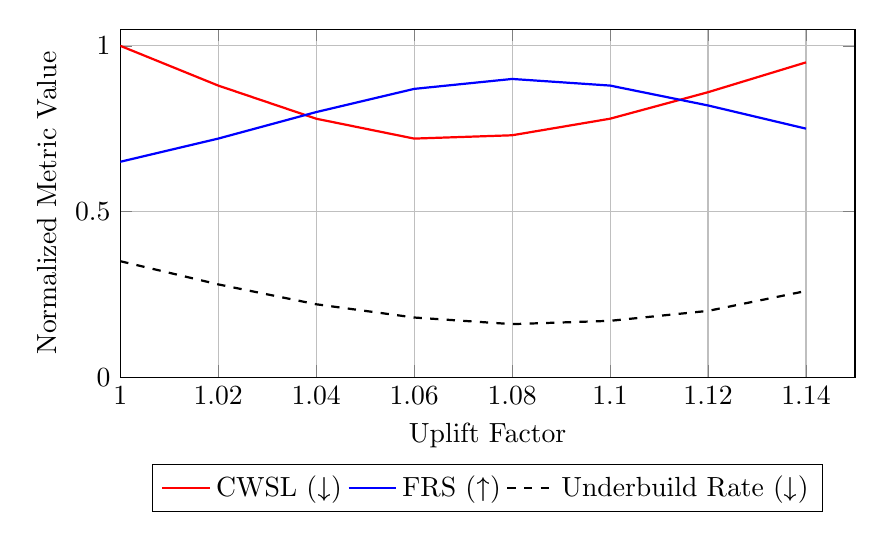
\begin{tikzpicture}
\begin{axis}[
    width=0.9\textwidth,
    height=6cm,
    xlabel={Uplift Factor},
    ylabel={Normalized Metric Value},
    xmin=1.0, xmax=1.15,
    ymin=0, ymax=1.05,
    legend style={at={(0.5,-0.25)}, anchor=north, legend columns=3},
    grid=major,
]

% CWSL (lower is better)
\addplot[thick, red]
coordinates {
    (1.00, 1.00)
    (1.02, 0.88)
    (1.04, 0.78)
    (1.06, 0.72)
    (1.08, 0.73)
    (1.10, 0.78)
    (1.12, 0.86)
    (1.14, 0.95)
};
\addlegendentry{CWSL (↓)}

% FRS (higher is better)
\addplot[thick, blue]
coordinates {
    (1.00, 0.65)
    (1.02, 0.72)
    (1.04, 0.80)
    (1.06, 0.87)
    (1.08, 0.90)
    (1.10, 0.88)
    (1.12, 0.82)
    (1.14, 0.75)
};
\addlegendentry{FRS (↑)}

% Underbuild Rate (lower is better)
\addplot[thick, dashed, black]
coordinates {
    (1.00, 0.35)
    (1.02, 0.28)
    (1.04, 0.22)
    (1.06, 0.18)
    (1.08, 0.16)
    (1.10, 0.17)
    (1.12, 0.20)
    (1.14, 0.26)
};
\addlegendentry{Underbuild Rate (↓)}

\end{axis}
\end{tikzpicture}
\caption{
Illustrative tradeoffs between cost-weighted service loss (CWSL),
Forecast Readiness Score (FRS), and underbuild rate as a function of
the uplift factor within a bounded feasibility envelope.
}
\label{fig:ral_uplift_tradeoff}
\end{figure}

The tradeoffs induced by the adjustment rule are illustrated in
Figure~\ref{fig:ral_uplift_tradeoff}. As the uplift factor varies within the
feasible envelope, cost-weighted service loss, forecast readiness, and
underbuild rate respond differently and exhibit opposing trends. Moderate
uplift reduces underbuild frequency and improves readiness, yielding a
corresponding reduction in decision-relevant loss. Beyond this region,
additional uplift increases overbuild cost and degrades overall performance.

RAL selects an operating point within this tradeoff surface that reduces
decision-relevant loss while preserving readiness and limiting adverse side
effects, rather than optimizing any single metric in isolation.

\subsection{Identity Condition}

If no adjustment within the feasible set produces a reduction in cost-weighted
service loss, RAL defaults to the identity transformation,
\[
\yhatadj = \yhat.
\]
This condition ensures that RAL cannot degrade performance relative to the
baseline forecast under the specified loss function and constraints.

\subsection{Outputs}

The primary output of RAL is the adjusted forecast \(\yhatadj\). In addition,
RAL produces diagnostic quantities used for evaluation and audit, including:
\begin{itemize}[leftmargin=*]
    \item Change in loss,
    \(\DeltaCWSL = \CWSL(\yhatadj) - \CWSL(\yhat)\).
    \item Change in Forecast Readiness Score (FRS), capturing improvements in
    readiness under asymmetric cost.
    \item Changes in under-readiness indicators, such as the underbuild rate
    \(\UBR\).
\end{itemize}

In addition to loss reduction, these diagnostics enable multi-metric audit of
readiness improvement and potential side effects, ensuring that RAL enhances
operational readiness rather than exploiting a single loss function. The
availability of parallel loss, readiness, and underbuild signals preserves
interpretability, supports governance review, and provides traceability for
downstream decision-making.
% ----------------------------------------------------------
% OPERATIONAL MOTIVATION
% ----------------------------------------------------------
\section{Operational Motivation}

Many operational workflows exhibit strong directional asymmetry in the
consequences of forecast error. A modest underforecast during a peak period may
lead to lost throughput, service degradation, queueing instability, or cascading
delays. By contrast, a modest overforecast is often absorbed through buffers,
inventory, slack labor capacity, or unused production bandwidth. This directional
imbalance in the operational impact of forecasting error reflects a longstanding
theme in decision-oriented forecasting research, where asymmetric loss functions
are used to represent unequal consequences of over- and underprediction
\citep{zellner1986}. As a result, operators are typically more sensitive to the
\emph{cost consequences} of error than to its numerical magnitude alone.

Cost-Weighted Service Loss (\CWSL) encodes these consequences directly. By
assigning explicit penalty weights to shortfall and overbuild magnitudes, the
metric enables evaluation in environments where:

\begin{itemize}
    \item underbuilding leads to operational or financial loss,
    \item overbuilding introduces secondary inefficiencies but is less harmful,
    \item the relative severity of these effects is understood or can be estimated,
    \item comparisons must remain meaningful across heterogeneous items, locations,
          or dayparts.
\end{itemize}

Traditional symmetric error metrics cannot express these realities. They treat
positive and negative deviations equivalently and therefore obscure whether a
forecast poses operational risk. In contrast, \CWSL{} provides a cost-aligned
view of error by quantifying the \emph{effective fraction of demand lost} under
the chosen penalty structure. This makes the metric particularly well suited to
readiness-oriented forecasting contexts—those in which the consequences of being
short or long differ materially and must be reflected in model evaluation.
% ----------------------------------------------------------
% PROPERTIES AND BEHAVIOR
% ----------------------------------------------------------
\section{Properties and Behavior}

The Forecast Readiness Score (\FRS) inherits interpretable and operationally
meaningful behavior from its two constituent components—\NSL{} and the scaled
cost term \CWSLscaled{}. This section summarizes the key mathematical and
practical properties governing how the score responds to different patterns of
forecast error.

\subsection{Boundedness}

Because both \NSL{} and \CWSLscaled{} lie in \([0,1]\), their difference satisfies:
\[
-1 \;\le\; \FRS = \NSL - \CWSLscaled \;\le\; 1.
\]

This bounded range facilitates clear interpretation and consistent comparison
across forecasting systems.

\subsection{Monotonicity}

\FRS{} behaves monotonically with respect to its components:

\begin{itemize}
    \item Increasing \NSL{} increases \FRS.
    \item Increasing \CWSL{} (and therefore \CWSLscaled{}) decreases \FRS.
    \item With identical \NSL{}, the forecast with lower \CWSL{} has the higher \FRS.
    \item With identical \CWSL{}, the forecast with higher \NSL{} has the higher \FRS.
\end{itemize}

These relationships ensure that \FRS{} respects intuitive operational
preferences: reliability is rewarded, and cost exposure is penalized.

\subsection{Sensitivity to Error Types}

\FRS{} differentiates sharply between shortfalls and overbuild errors:

\begin{enumerate}
    \item \textbf{Shortfalls} reduce \NSL{} and increase \CWSL{}, typically causing
    significant declines in \FRS.
    \item \textbf{Overbuild errors} leave \NSL{} unchanged but increase \CWSLscaled{},
    producing more moderate reductions in \FRS.
\end{enumerate}

This structural asymmetry reflects real operational priorities, where shortfalls
create significantly higher service and cost risk.

\begin{figure}[htbp]
\centering
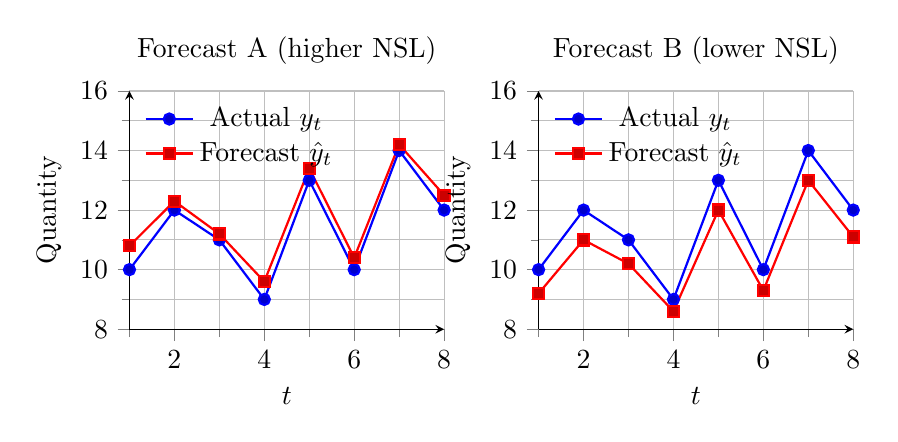
\begin{tikzpicture}
\begin{groupplot}[
    group style={group size=2 by 1, horizontal sep=1.2cm},
    width=0.46\linewidth,
    height=0.38\linewidth,
    xmin=1, xmax=8,
    ymin=8, ymax=16,
    xlabel={$t$},
    ylabel={Quantity},
    axis lines=left,
    grid=both,
    minor tick num=1,
    tick align=outside,
    legend style={draw=none, fill=none, at={(0.02,0.98)}, anchor=north west},
]

\nextgroupplot[title={Forecast A (higher NSL)}]
\addplot+[thick, mark=*] coordinates {(1,10) (2,12) (3,11) (4,9) (5,13) (6,10) (7,14) (8,12)};
\addlegendentry{Actual $y_t$}
\addplot+[thick, mark=square*] coordinates {(1,10.8) (2,12.3) (3,11.2) (4,9.6) (5,13.4) (6,10.4) (7,14.2) (8,12.5)};
\addlegendentry{Forecast $\hat{y}_t$}

\nextgroupplot[title={Forecast B (lower NSL)}]
\addplot+[thick, mark=*] coordinates {(1,10) (2,12) (3,11) (4,9) (5,13) (6,10) (7,14) (8,12)};
\addlegendentry{Actual $y_t$}
\addplot+[thick, mark=square*] coordinates {(1,9.2) (2,11.0) (3,10.2) (4,8.6) (5,12.0) (6,9.3) (7,13.0) (8,11.1)};
\addlegendentry{Forecast $\hat{y}_t$}

\end{groupplot}
\end{tikzpicture}
\caption{Illustration of FRS sensitivity to error type. Two forecasts can exhibit similar symmetric accuracy (e.g., RMSE/MAE) while differing materially in shortfall behavior and asymmetric cost exposure, producing different FRS values.}
\label{fig:frs_sensitivity}
\end{figure}

\subsection{Smoothness and Stability}

Because \CWSL{} is a continuous function of the forecast and \NSL{} is a
step function, \FRS{} exhibits the following behaviors:

\begin{itemize}
    \item \FRS{} is piecewise continuous, with discontinuities arising only when
    \(\hat{y}_t\) crosses \(y_t\), changing the shortfall indicator.
    \item Small forecast adjustments that do not change shortfall occurrence
    produce smooth changes in \FRS.
    \item Structural shifts (such as systematic underforecasting) induce
    predictable, interpretable shifts in both \NSL{} and \CWSL{}, resulting in
    corresponding changes in \FRS.
\end{itemize}

\subsection{Response to Systematic Bias}

\FRS{} responds asymmetrically to forecast bias:

\begin{itemize}
    \item \textbf{Underforecast bias} reduces \NSL{} and increases \CWSL{},
    resulting in sharp decreases in \FRS.
    \item \textbf{Overforecast bias} preserves \NSL{} but increases \CWSL{},
    reducing \FRS{} more gradually.
\end{itemize}

This behavior aligns with operational reality in environments where shortages
carry disproportionately greater cost than excess production.

\subsection{Perfect Forecasts}

If the forecast matches actual demand in every interval
(\(\hat{y}_t = y_t\)), then:
\[
\NSL = 1, \qquad \CWSL = 0, \qquad \CWSLscaled = 0,
\]
so that:
\[
\FRS = 1.
\]

\subsection{Extreme Miscalibration}

If a forecasting system persistently underbuilds demand, then:
\[
\NSL \approx 0, \qquad \CWSLscaled \approx 1,
\]
and thus:
\[
\FRS \approx -1.
\]

Such values signal a severe readiness deficit and a forecasting system misaligned
with operational service and cost requirements.
% ----------------------------------------------------------
% ILLUSTRATIVE EXAMPLE
% ----------------------------------------------------------
\section{Illustrative Example}

To illustrate the behavior of Cost-Weighted Service Loss (\CWSL), consider a
single entity evaluated over twelve intervals. Consistent with many operational
settings where underforecasting is more harmful than overforecasting, we adopt
an asymmetric penalty structure with
\[
\cu = 2, 
\qquad 
\co = 1.
\]

Table~\ref{tab:cwsl_example} reports realized demand \(y_t\), forecast values
\(\hat{y}_t\), raw errors \(e_t = \hat{y}_t - y_t\), and the corresponding
cost-weighted contributions for each interval.

\begin{table}[h!]
\centering
\begin{tabular}{c c c c c}
\toprule
Interval $t$ & $y_t$ & $\hat{y}_t$ & Error $e_t$ & CWSL Contribution \\
\midrule
1  & 20 & 22 &  \phantom{-}2 & $c^o \cdot 2 = 2$ \\
2  & 28 & 25 & -3            & $c^u \cdot 3 = 6$ \\
3  & 32 & 29 & -3            & $c^u \cdot 3 = 6$ \\
4  & 35 & 36 &  \phantom{-}1 & $c^o \cdot 1 = 1$ \\
5  & 40 & 37 & -3            & $c^u \cdot 3 = 6$ \\
6  & 42 & 45 &  \phantom{-}3 & $c^o \cdot 3 = 3$ \\
7  & 38 & 34 & -4            & $c^u \cdot 4 = 8$ \\
8  & 30 & 31 &  \phantom{-}1 & $c^o \cdot 1 = 1$ \\
9  & 26 & 22 & -4            & $c^u \cdot 4 = 8$ \\
10 & 24 & 27 &  \phantom{-}3 & $c^o \cdot 3 = 3$ \\
11 & 22 & 23 &  \phantom{-}1 & $c^o \cdot 1 = 1$ \\
12 & 18 & 19 &  \phantom{-}1 & $c^o \cdot 1 = 1$ \\
\bottomrule
\end{tabular}
\caption{Cost-weighted contributions for a 12-interval example under a 
penalty structure with $c^u = 2$ and $c^o = 1$.}
\label{tab:cwsl_example}
\end{table}

Summing across intervals, the total cost-weighted deviation is
\[
\text{Numerator} 
= 2 + 6 + 6 + 1 + 6 + 3 + 8 + 1 + 8 + 3 + 1 + 1 
= 46.
\]

The denominator is total realized demand:
\[
\text{Denominator}
= \sum_{t=1}^{12} y_t
= 20 + 28 + 32 + 35 + 40 + 42 + 38 + 30 + 26 + 24 + 22 + 18
= 357.
\]

Thus, the Cost-Weighted Service Loss for this example is
\[
\CWSL
= \frac{46}{357}
\approx 0.129.
\]

\subsection*{Interpretation}

A \CWSL{} value of approximately \(0.129\) indicates that, under the assumed cost
structure, the forecast produced cost-weighted deviations equivalent to losing
roughly 13\% of realized throughput. Despite several intervals with small
overbuilds, the repeated underbuild events—magnified by the higher shortfall
penalty—dominate the loss. This example illustrates how \CWSL{} highlights
directional operational risk even when symmetric error metrics (e.g., RMSE or
MAE) may appear moderate.
% ----------------------------------------------------------
% USE CASES
% ----------------------------------------------------------
\section{Use Cases Across Operational Domains}

The Forecast Readiness Score (\FRS) supports decision-making in environments
where service reliability, asymmetric cost considerations, and execution
feasibility are more important than purely statistical accuracy. Because \FRS{}
summarizes both shortfall avoidance and cost-efficient performance, it is
well-suited for operational forecasting workflows that require interpretable
readiness diagnostics. Importantly, \FRS{} is intended as an evaluative signal of
forecast readiness rather than a direct optimization target or execution rule.

\subsection{Short-Horizon Demand Planning}

In short-horizon production, retail replenishment, and perishable inventory
settings, operational disruption is driven primarily by \emph{shortfalls}.
Small overbuilds are often absorbable, but even a modest number of shortfall
intervals can degrade service or throughput. \FRS{} is valuable here because:

\begin{itemize}
    \item \NSL{} captures how frequently demand is fully covered,
    \item \CWSLscaled{} penalizes shortfalls more heavily than excess,
    \item the composite score reflects readiness to execute without service failure.
\end{itemize}

These properties make \FRS{} a natural KPI for short-horizon service reliability.

\subsection{Labor and Capacity Planning}

In staffing, labor scheduling, and capacity planning environments (e.g.,
restaurants, logistics centers, call centers), underforecasts degrade service
quality by generating long queues, slow response times, or labor shortages.
Overstaffing, while inefficient, is typically less harmful than understaffing.

\FRS{} provides a principled framework to:

\begin{itemize}
    \item incorporate asymmetric cost assumptions through the \((\cu, \co)\) parameters,
    \item quantify readiness to meet workload requirements,
    \item compare alternative forecast models under realistic operational criteria.
\end{itemize}

\subsection{Model Selection and Deployment Decisions}

\FRS{} can serve as a primary metric for choosing among competing forecasting
models. Because it encodes operational feasibility rather than purely numerical
accuracy, it helps prevent situations in which a statistically optimal model
performs poorly once deployed.

Applications include:

\begin{itemize}
    \item validation-set model comparison,
    \item production monitoring of forecast degradation,
    \item regression testing after model retraining.
\end{itemize}

\subsection{Segmented and Entity-Level Evaluation}

Operational environments often exhibit heterogeneous behavior across products,
locations, time blocks, or customer segments. \FRS{} can be computed:

\begin{itemize}
    \item globally (system-wide readiness),
    \item per entity (e.g., per SKU or store),
    \item per segment (e.g., store clusters, product families).
\end{itemize}

This enables targeted diagnosis of readiness gaps and supports interventions
tailored to specific segments.

\subsection{Operational Monitoring and Governance}

Because \FRS{} is bounded and interpretable, it can function as an operational
KPI within forecasting governance frameworks. Declines in \FRS{} over time signal:

\begin{itemize}
    \item increasing shortfall frequency,
    \item rising asymmetric error costs,
    \item erosion of deployment readiness.
\end{itemize}

This makes \FRS{} useful for ongoing monitoring, alerting, and readiness audits
in production forecasting systems.

% ----------------------------------------------------------
% LIMITATIONS
% ----------------------------------------------------------
\section{Limitations and Appropriate Use}

Although \UD\ provides a focused measure of shortfall severity, several limitations
should guide its interpretation and application. In particular, \UD\ is intended
as an evaluative diagnostic of underbuild depth and should not be optimized in
isolation or treated as a prescriptive control target; it is most informative
when interpreted alongside complementary frequency- and balance-based metrics.

\subsection{Undefined When No Shortfalls Occur}

When no shortfall intervals are observed, \UD\ is undefined because there is no
depth to average. Implementations may return zero or a missing value depending on
whether the distinction between ``no shortfalls'' and ``no depth'' is
operationally meaningful.

\subsection{No Frequency Information}

\UD\ measures severity rather than incidence. Forecasting systems with identical
\UD\ values may exhibit very different frequencies of shortfalls. For a complete
assessment of forecast readiness, \UD\ should be paired with coverage-based
metrics.

\subsection{Scale Dependence}

Because \UD\ reflects the magnitude of unmet demand, it is sensitive to the scale
of the underlying process. Comparisons across entities with different demand
levels require normalization or supplemental diagnostics.

\subsection{Sensitivity to Rare Extremes}

A small number of deep shortfalls can disproportionately elevate \UD. While this
behavior is often desirable for risk identification, it should be interpreted
carefully in noisy or highly volatile environments.

\subsection{No Information on Overbuilding}

\UD\ does not capture surplus capacity or overforecasting behavior. Evaluations
concerned with the balance between underbuilding and overbuilding require
additional metrics.

\subsection{Dependence on Interval Resolution}

The choice of interval length affects the metric. Shorter intervals may reveal
localized deep shortfalls, while longer intervals may obscure them. \UD\ should be
computed at the operational decision cadence relevant to the system being
evaluated.

% ----------------------------------------------------------
% CONCLUSION
% ----------------------------------------------------------
\section{Conclusion}

Cost-Weighted Service Loss (\CWSL) provides a principled, operationally aligned
approach to evaluating forecast performance in environments where the
consequences of under- and overforecasting differ meaningfully. By applying
explicit penalty weights to shortfall and overbuild magnitudes and normalizing
by realized demand, \CWSL{} quantifies the effective fraction of throughput
“lost’’ due to misalignment between forecasted and actual values. This
interpretation makes the metric especially useful in high-frequency,
readiness-oriented contexts where service reliability and cost exposure must be
managed jointly.

\CWSL{} complements traditional symmetric accuracy metrics by emphasizing the
\emph{cost of error} rather than its purely numerical magnitude. As a result, it
provides insight into operational risk that may remain hidden when evaluation
relies solely on RMSE, MAE, or related measures. When paired with
frequency-based diagnostics, distributional analysis, and readiness-focused
metrics, \CWSL{} helps create a richer and more actionable understanding of
forecasting system performance.

As organizations increasingly rely on automated forecasting for production,
staffing, logistics, replenishment, and energy management, metrics such as
\CWSL{} enable more transparent decision-making and more resilient operational
planning. Future extensions may include probabilistic formulations, integration
with scenario-based cost models, or dynamic adjustment of penalty weights to
reflect changing conditions or risk preferences. Together, these developments
further extend the connection between statistical forecasting and the operational
realities it must ultimately support.

% ----------------------------------------------------------
% REFERENCES
% ----------------------------------------------------------
\bibliographystyle{plainnat}
\bibliography{references}

\end{document}